\chapter{FHTBoost: A twodimensional component-wise gradient boosting algorithm for survival data}
\label{ch:FHTboost}
In this chapter, we propose a component-wise boosting algorithm for fitting the inverse Gaussian first hitting time (FHT) model (section \ref{sec:FHT} and onward) to survival data.
We work with survival data sets with $N$ observations,
\begin{equation}\label{eq:data-fhtboost}
    D=(\x_i,\z_i,t_i,d_i)_{i=1}^N.
\end{equation}
Here $t_i$ is a possibly right-censored event time, $d_i$ is an indicator variable which is 1 if $t_i$ is an actually observed event time, and 0 if it is right-censored.
For simplicity, we sometimes denote the response data
\begin{equation*}
    y_i=(t_i,d_i).
\end{equation*}
Further, we have $\x_i$ and $\z_i$, covariate vectors that will be related to the inverse Gaussian parameters $y_0$ and $\mu$, respectively.
$\x_i$ is defined as
\begin{equation}
    \x_i=(x_{i,1},x_{i,2},\ldots,x_{i,p_1}),
\end{equation}
with $p_1$ number of covariates, and $\z_i$ is defined as
\begin{equation}
    \z_i=(z_{i,1},z_{i,2},\ldots,z_{i,p_2}),
\end{equation}
with $p_2$ number of covariates.
The dimensions of the matrices, $p_1$ and $p_2$, can be any size.
There are theoretical arguments for this particular combination of the high and low-dimensional vectors and parameters, which we have discussed earlier in subsection \ref{subsec:FHT-combine}.
Before describing the algorithm in detail, we explain the necessary parts and expressions that will be used in the algorithm.

\section{Setting}
\subsection{Additive predictors}
The first-hitting-time model with Wiener processes, as shown, leads to inverse Gaussian lifetimes.
The log likelihood is given in \eqref{eq:loglik}, but we repeat it here.
It depends on $y_0$, $\mu$, and $\sigma$, but in practice $\sigma$ is set to 1 to avoid overparameterization (see subsection \ref{subsec:overdetermined} for reasoning).
Given a data set $D$ \eqref{eq:data-fhtboost}, the log-likelihood of the parameters given $D$ is
\begin{align*}
\begin{split}
    l(y_0,\mu|y_i)=\sum_{i=1}^N&d_i\p*{\ln y_0-\frac{1}{2}\ln\p*{2\pi\ti^3}-\frac{\p*{\mu\ti+y_0}^2}{2\ti}} \\
    &+
    (1-d_i)\ln\p*{\Phi\p*{\frac{\mu\ti+y_0}{\sqrt{\ti}}}-\exp\p*{-2y_0\mu}\Phi\p*{\frac{\mu\ti-y_0}{\sqrt{\ti}}}}.
\end{split}
\end{align*}
We denote the $K=2$ distribution parameters as
\begin{equation*}
    \btheta=(\theta_1,\theta_2)^T=(y_0,\mu).
\end{equation*}
We wish to use a similar setup as the GAMLSS (see subsection \ref{subsec:GAMLSS}).
We will therefore model the parameters through additive predictors $\eta_1$ and $\eta_2$.
We relate the additive predictors to covariates, and further relate the additive predictors to the parameters by their usual link functions, i.e. the log link for $y_0$ (to ensure it is positive) and just the identity link for the drift $\mu$.
In FHT regression, the additive predictors are typically \textit{linear} predictors.
We also choose to use this.
The additive predictors for an individual $i$ are defined as
\begin{equation}\label{eq:eta1}
    \eta_{1,i}\coloneqq \ln(y_{0,i})=\bbeta^T \x_i=\beta_{0}+\sum_{j=1}^{p_1}x_{j,i}\beta_j
\end{equation}
and
\begin{equation}\label{eq:eta2}
    \eta_{2,i}\coloneqq \mu_{i}=\bgamma^T \z_i=\gamma_{0}+\sum_{j=1}^{p_2}z_{j,i}\gamma_j,
\end{equation}
and we denote the vector containing both as $\boldeta_i=\left(\eta_{1,i},\eta_{2,i}\right)$.
We are going to build up these additive predictors by means of gradient boosting.
Choosing a linear structure for the additive predictors means we need to choose base learners in the boosting algorithm which allows for this.

\subsection{Base learners}
To use additive predictors we need base learners that add up to the additive structure of \eqref{eta1} and \eqref{eta2}.
We therefore choose regular least squares functions of only one covariate.
Each base learner is a function of an observation $i$, but only uses one covariate in each.
This is common in gradient boosting algorithms \citep{gamboost}.
This means that the base learners corresponding to $\eta_1$, $\{h_{1,j}\}_{j=1}^{p_1}$ as a function of $\x_i$ is
\begin{equation*}
    \{h_{1,j}(\x_i)\}_{j=1}^{p_1}=\{h_{1,j}(x_{i,j})\}_{j=1}^{p_1}=\{\beta_jx_{i,j}\}_{j=1}^{p_1}.
\end{equation*}
To estimate a base learner $\hat{h}_{1,j}$, we use ordinary least squares to calculate $\hat{\beta}_j$.
The vector that we wish to fit is $\u_1$, the vector of generalized residuals for parameter $y_0$.
The estimated parameter $\hat{\beta}_j$ will therefore be
\begin{equation*}
    \hat{\beta}_j=\left(\x_j^T\x_j\right)^{-1}\x_j^T \u_1=\frac{\sum_{k=1}^N u_{1,k}x_{k,j}}{\sum_{k=1}^N x_{k,j}^2}.
\end{equation*}
The estimated base learner $\hat{h}_j$, as a function of an observation $\x_i=(x_{i,1},x_{i,2},\ldots,x_{i,j},\ldots,x_{i,N})$ is thus
\begin{equation*}
    \hat{h}_{1,j}(\x_i)=\hat{\beta_j}x_{i,j}=\frac{\sum_{k=1}^N u_{1,k}x_{k,j}}{\sum_{k=1}^N x_{k,j}^2}x_{i,j}.
\end{equation*}
Similarly, the base learners for $\eta_2$, are $\{h_{2,j}\}_{j=1}^{p_1}$.
Each $h_{2,j}(\cdot)$ uses covariate $j$ from the $\z_j$ vector of covariates.
As a function of one observation $\z_i$, it is given by
\begin{equation*}
    \{h_{2,j}(\z_i)\}_{j=1}^{p_1}=\{h_{2,j}(z_{i,j})\}_{j=1}^{p_1}=\{\gamma_jz_{i,j}\}_{j=1}^{p_1}.
\end{equation*}
To estimate $\hat{\gamma}$, the same method is used as for $\hat{\beta}$, namely to calculate the ordinary least squares parameter, but here the response is $\u_2$, the generalized residuals for parameter $\mu$.
An estimated base learner $h_{2,j}$ for an observation $\z_i$ is
\begin{equation*}
    \hat{h}_{2,j}(\z_i)=\hat{\gamma}_jz_{i,j}=\frac{\sum_{k=1}^N u_{2,k}z_{k,j}}{\sum_{k=1}^N z_{k,j}^2}z_{i,j}.
\end{equation*}
In each boosting iteration, all base learners $h_{1,j}$ and each covariate $j=1,\ldots,p_1$ as well as all base learners $h_{2,j}$ and each covariate $j=1,\ldots,p_2$ are estimated.
The best fitting base learner for each $k=1,2$ is calculated, and then the one of these two that leads to best decrease in the training error, is added to the boosted model.

\subsection{Resulting model after boosting}
After $\mstop$ iterations, we have additive predictors $\hat{\eta}_1^{[\mstop]}$ and $\hat{\eta}_2^{[\mstop]}$.
As a sum of the boosted additions, they are
\begin{equation*}
    \hat{\eta}_1^{[\mstop]}(\x)=\hat{\beta_0}+\sum_{m=1}^{\mstop}\nu\cdot \hat{h}_{j^{[m]}}^{[m]}(\x)
\end{equation*}
and
\begin{equation*}
    \hat{\eta}_2^{[\mstop]}(\z)=\hat{\gamma}_0+\sum_{m=1}^{\mstop}\nu\cdot \hat{h}_{j^{[m]}}^{[m]}(\z).
\end{equation*}
They can also be seen as linear predictors of the form \eqref{eq:eta1} and \eqref{eq:eta2},
\begin{equation*}
    \hat{\eta}_1^{[\mstop]}(\x)=\hat{\bbeta}^T\x=\hat{\beta}_0+\sum_{j=1}^{p_1}\hat{\beta}_jx_j
\end{equation*}
and
\begin{equation*}
    \hat{\eta}_2^{[\mstop]}(\z)=\hat{\bgamma}^T\z=\hat{\gamma}_0+\sum_{j=1}^{p_2}\hat{\gamma}_jz_j.
\end{equation*}
Here the parameters $\hat{\beta}_0$ and $\hat{\gamma}_0$ are the intercepts calculated initially.
Further, the parameters for covariates, $\hat{\beta}_j$ and $\hat{\gamma}_j$, are sums of the boosted parameters, i.e.,
\begin{equation*}
    \hat{\beta}_j=\nu\sum_{m=1}^{[\mstop]}\indicator\left(j_1^{[m]}=j\right)\hat{\beta}_j^{[m]},
\end{equation*}
for $j=1,\ldots,p_1$, and
and
\begin{equation*}
    \hat{\gamma}_j=\nu\sum_{m=1}^{[\mstop]}\indicator\left(j_2^{[m]}=j\right)\hat{\gamma}_j^{[m]},
\end{equation*}
for $j=1,\ldots,p_2$.



\subsection{Loss function}
Since we assume we have observations from a probability distribution, we should use the negative of the corresponding log likelihood as our loss function \citep{mayr14a}.
In general, for an observation $y$, and parameters $y_0$ and $\mu$, the loss function is
\begin{equation*}
    \rho(y,\btheta)=-l(y_{0},\mu|y).
\end{equation*}
For an observation numbered $i$, an estimate of its parameter vector is
\begin{equation*}
    \hat{\btheta}_i=\left(\hat{y}_{0,i},\hat{\mu}_i\right).
\end{equation*}
Given an estimated additive predictor $\hat{\boldeta}$, we calculate the corresponding estimated distribution parameters by transforming the additive predictors via the inverse of their link functions.
Thus,
\begin{equation}
    \hat{y}_{0,i}=\hat{\theta}_{1,i}=g_1^{-1}(\hat{\eta}_{1,i})=\exp(\hat{\eta}_{1,i}),
\end{equation}
and
\begin{equation}
    \hat{\mu}_i=\hat{\theta}_{2,i}=g_2^{-1}(\hat{\eta}_{2,i})=\hat{\eta}_{2,i}.
\end{equation}
This means that as a function of the additive predictors, the loss function for an observation $i$ is
\begin{equation*}
    \rho(y_i,\hat{\boldeta}_i)=-l(\exp(\hat{\eta}_{1,i}), \hat{\eta}_{2,i}),
\end{equation*}
where $l$ again is the log-likelihood.
To use the gradient boosting algorithm, we need to compute the negative gradient of the loss function, i.e., the negative of the derivative. 
The negative partial derivative of the loss function is just the partial derivative of the log-likelihood function.
These are
\begin{equation}
    -\frac{\partial}{\partial\eta_1}\rho(y_i,\hat{\btheta}_i)=\frac{\partial}{\partial\eta_1}l(\exp(\hat{\eta}_{1,i}), \hat{\eta}_{2,i})=f_1
\end{equation}
and
\begin{equation}
    -\frac{\partial}{\partial\eta_2}\rho(y_i,\hat{\btheta}_i)=\frac{\partial}{\partial\eta_2}l(\exp(\hat{\eta}_{1,i}), \hat{\eta}_{2,i})=f_1
\end{equation}
We can now apply the component-wise multidimensional boosting algorithm shown in the previous chapter.

\subsection{Choice of noncyclical vs cyclical}
We choose to use the noncyclical variant as this leads to equally good results and is less computationally intensive to tune, due to a one-dimensinal stopping parameter search, as stated in \citet{schmid}.

\section{Initialization via maximum likelihood estimate}
To ensure proper estimation of $\eta_1$ and $\eta_2$, we need to compute the intercepts $\beta_{0}$ and $\gamma_{0}$, which capture the general, average effect of the covariates.
If analytical relationships or formulas exist, such as taking the average of a Gaussian distributed variable in an ordinary regression setting, their computation would be straightforward.
In lieu of such known formulas, a reasonable method to use is to perform numerical maximization of the log-likelihood, treating the log likelihood as a function of
\begin{equation*}
    \boldeta_0=\left(\beta_{0},\gamma_{0}\right)
\end{equation*}
only.
Hence the intercepts are estimated to be
\begin{equation*}
    \hat{\boldeta}_0=\argmin_{\boldeta}\err\left(\boldeta\right).
\end{equation*}
To do this in practice, we use the routine called \verb|nlm|, which belongs to the base package of \verb|R| \citep{Rlang}.
As our base learners are only functions with parametric effects and no intercept, these intercepts are fixed throughout.

\begin{algorithm}
\section{The FHTBoost algorithm with fixed intercepts}
\label{algo:fhtboost}
\begin{enumerate}
    \item
        Given a survival data set $D=(\x_i, \z_i, t_i,d_i)_{i=1}^N$, where for each observation $i$,
        $\x_i$ and $\z_i$ are vectors of covariate information,, $t_i$ is the possibly right-censored survival time, and $d_i$ is the censoring indicator.
        We wish to estimate the $\hat{\boldeta}$ that minimizes the training error in $\mstop$ number of iterations,
        \begin{equation*}
            \hat{\boldeta}=\argmin_{\boldeta}\err(\boldeta)
        \end{equation*}
    \item
        Set iteration counter $m$ to $0$.
        Specify stopping iteration $\mstop$.
        Initialize additive predictors $\hat{\boldeta}_0=\left(\beta_{0},\gamma_{0}\right)$, by finding maximum likelihood constants through numerical maximization,
        \begin{equation*}
            \hat{\boldeta}_0=\argmin_{\boldeta}\err\left(\boldeta\right).
        \end{equation*}
    \item
    \label{algostep:FHT-base-learner}
        Specify linear least squares base learners:
        \begin{align*}
            \mathcal{H}_1&=\{h_{1,j}\}_{j=1}^{p_1}=\{x_j\beta_j\}_{j=1}^{p_1}, \\
            \mathcal{H}_2&=\{h_{2,j}\}_{j=1}^{p_1}=\{z_j\gamma_j\}_{j=1}^{p_2}
        \end{align*}
    \item
    \label{algostep:FHT-init}
        Increase $m$ by 1.
    \item
        Compute the negative partial derivative $-\frac{\partial\rho}{\partial \hat{\eta}_1}$
        and evaluate at $\hat{\boldeta}^{[m-1]}(\x_i,\,\z_i),i=1,\ldots,N$, yielding negative gradient vector
        \begin{equation*}
            \u^{[m-1]}_1=\left(-\frac{\partial}{\partial \hat{\eta}_1}\rho(y_i, \hat{\boldeta}^{[m-1]}(\x_i,\z_i))\right)_{i=1}^N
        \end{equation*}
    \item
        Fit the negative gradient vector to each of the $p_1$ components of $\X$ (i.e. to each base learner) separately, using the base learners specified in step \ref{algostep:FHT-base-learner}, so i.e., fitting
        \begin{equation*}
            \hat{\beta}_j^{[m]}=\left(\x_j^T\x_j\right)^{-1}\x_j^T \u^{[m-1]}_1=\frac{\sum_{k=1}^N u^{[m-1]}_{1,k}x_{k,j}}{\sum_{k=1}^N x_{k,j}^2},
        \end{equation*}
        and letting $\hat{h}_{1,j}^{[m]}(\x)=\hat{\beta}_j^{[m]}x_j$.
    \item
        Select the best fitting base learner, $\hat{h}_{1,\,j_1^{[m]}}$, by the inner loss,
        i.e., the RSS of the base-learner fit w.r.t the negative gradient vector
        \begin{equation*}
            j_1^{[m]}=\argmin_{j\in 1,\ldots,p_1}\sum_{i=1}^N\left(u_{1,i}^{[m-1]}-\hat{h}^{[m]}_{1,j}(\x_i)\right)^2.
        \end{equation*}
    \item
        Compute the possible improvement of this update regarding the outer loss,
        \begin{equation*}
            \Delta\rho_1=\err\left(\hat{\boldeta}^{[m-1]} + \nu \cdot \hat{h}^{[m]}_{1,\,j_1^{[m]}} \right)-\err\left(\hat{\boldeta}^{[m-1]} \right)
        \end{equation*}
    \item
        Compute the negative partial derivative $-\frac{\partial\rho}{\partial \hat{\eta}_2}$
        and evaluate at $\hat{\boldeta}^{[m-1]}(\x_i,\z_i),i=1,\ldots,N$, yielding negative gradient vector
        \begin{equation*}
            \u^{[m-1]}_1=\left(-\frac{\partial}{\partial \hat{\eta}_1}\rho(y_i, \hat{\boldeta}^{[m-1]}(\x_i,\z_i))\right)_{i=1}^N
        \end{equation*}
    \item
        Fit the negative gradient vector to each of the $p_2$ components of $\Z$ (i.e. to each base learner) separately, using the base learners specified in step \ref{algostep:FHT-base-learner}, so i.e., fitting
        \begin{equation*}
            \hat{\gamma}_j=\left(\z_j^T\z_j\right)^{-1}\z_j^T \u^{[m-1]}_2=\frac{\sum_{k=1}^N u^{[m-1]}_{2,k}z_{k,j}}{\sum_{k=1}^N z_{k,j}^2}.
        \end{equation*}
    \item
        Select the best fitting base learner, $\hat{h}^{[m]}_{2,j_2^{[m]}}$, by the inner loss,
        i.e., the RSS of the base-learner fit w.r.t the negative gradient vector
        \begin{equation*}
            j_2^{[m]}=\argmin_{j\in 1,\ldots,p_2}\sum_{i=1}^N\left(u_{2,i}^{[m-1]}-\hat{h}_{2,j}(\z_i)\right)^2.
        \end{equation*}
    \item
        Compute the possible improvement of this update regarding the outer loss,
        \begin{equation*}
            \Delta\rho_2=\err\left(\hat{\boldeta}^{[m-1]} + \nu \cdot \hat{h}^{[m]}_{2,\,j_2^{[m]}} \right)-\err\left(\hat{\boldeta}^{[m-1]}  \right)
        \end{equation*}
    \item
    \label{algostep:FHT-end}
        Find which parameter to include in the boosted model, i.e. the one with smallest gain in error,
        \begin{equation*}
            k^{[m]}=\argmin_{k\in\{1,2\}}\Delta\rho_k.
        \end{equation*}
        Include this component in the final model, by updating its additive predictor,
        \begin{equation*}
            \hat{\eta}^{[m]}_{k^{[m]}}\gets\hat{\eta}^{[m-1]}_{k^{[m]}}+\nu\cdot\hat{h}^{[m]}_{k^{[m]},\,j^{[m]}}(x),
        \end{equation*}
        while for the other component $k\neq k^{[m]}$, set the additive predictor for this iteration to be the same as previous iteration
        \begin{equation*}
            \hat{\eta}^{[m]}_{k}\gets\hat{\eta}^{[m-1]}_{k}.
        \end{equation*}
    \item
        If $m<m_{\text{stop}}$, go to step \ref{algostep:FHT-init}.
        If not, return
        \begin{equation*}
            \hat{\boldeta}(\cdot)=\hat{\boldeta}^{[\mstop]}(\cdot)=\hat{\boldeta}_0+\sum_{m=1}^{[\mstop]}\boldeta^{[m]}(\cdot).
        \end{equation*}
\end{enumerate}
\end{algorithm}

\section{Small example}
\label{subsec:algo-example}
Let us now consider a small example where we draw survival times from an inverse Gaussian FHT distribution \eqref{eq:ig-pdf}, and confirm that FHTBoost recovers the maximum likelihood parameters.
Let parameter vectors be
\begin{equation*}
    \bbeta=(2,0.1,0.2)
\end{equation*}
and
\begin{equation*}
    \bgamma=(-1, -0.1, 0.1)
\end{equation*}
We let the covariate matrices be $\X=(\x_1,\x_2)$ and $\Z=(\z_1,\z_2)$, where all elements in the covariate vectors $\x_1,\x_2,\z_1,\z_2$ are independently drawn from $N(0,1)$.
We simulate data using Algorithm \ref{algo:FHT-sim} in section \ref{sec:simulate-IG-data}, with censoring times $w_i$ being drawn from a distribution $\exp(0.1)$.
We thus end up with a survival data set of the by now usual form
\begin{equation*}
    D=(\x_i,\z_i,t_i,d_i)_{i=1}^N.
\end{equation*}
The resulting survival times have Kaplan-Meier estimates shown as the solid black line in Figure \ref{fig:small-example-kaplan-meier}.
\begin{figure}
\caption{Kaplan-Meier plot of generated survival data from subsection \ref{subsec:algo-example}.}
\label{fig:small-example-kaplan-meier}
\centering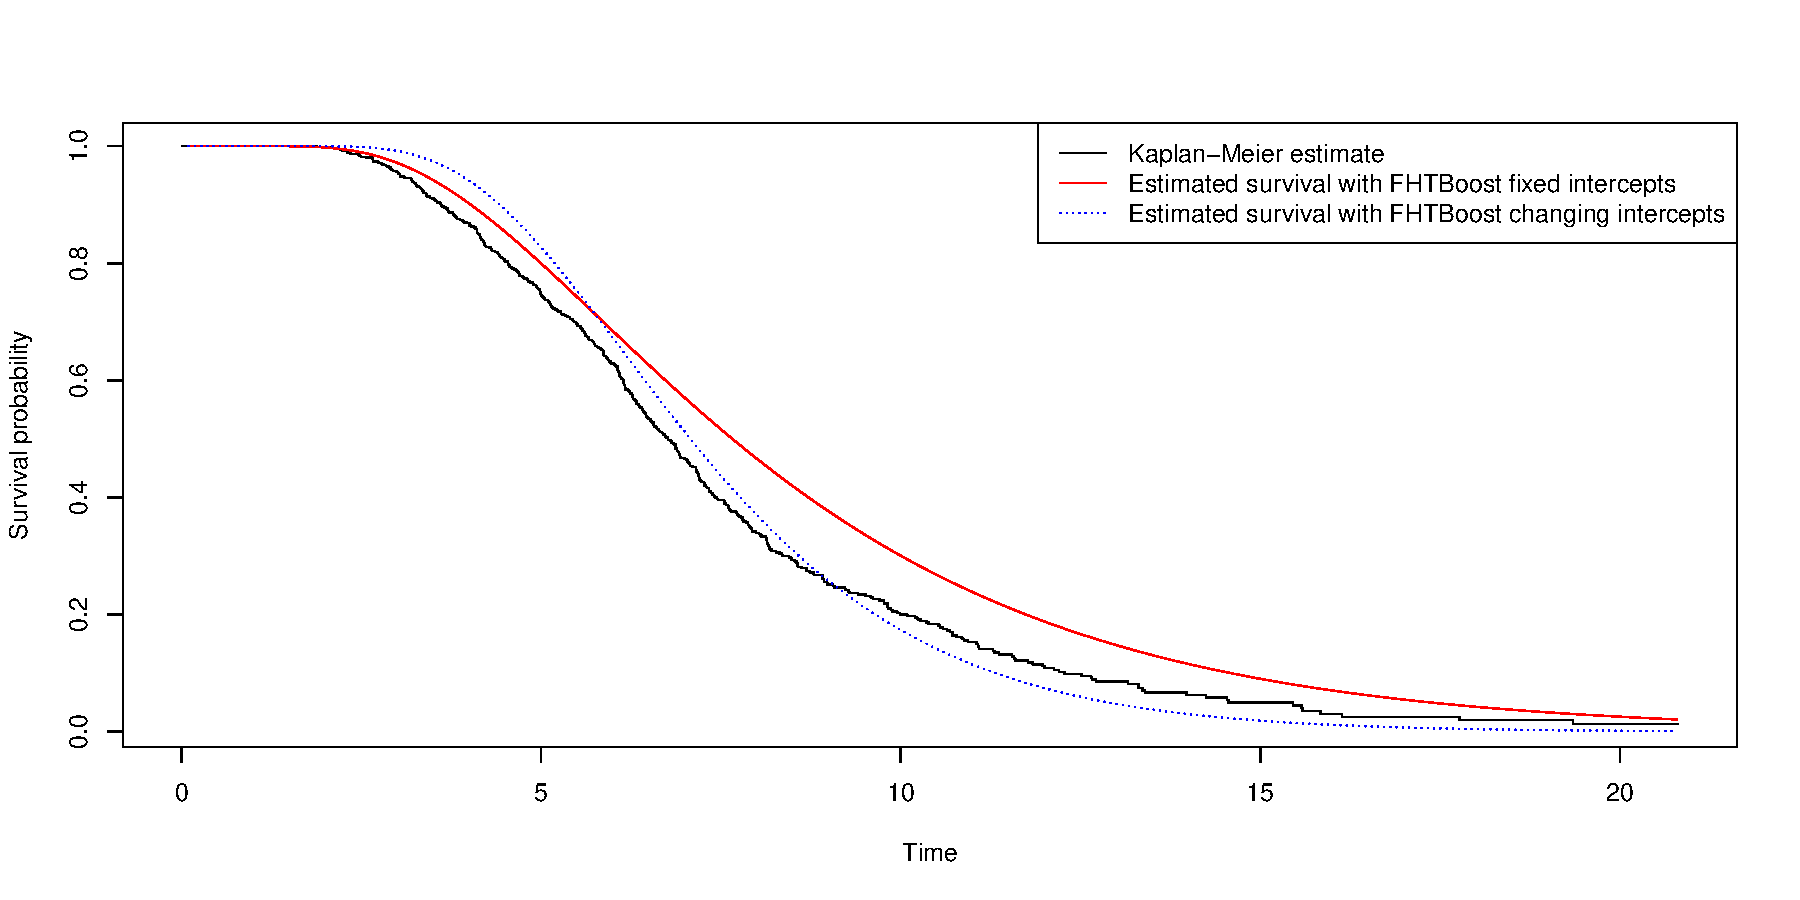
\includegraphics[scale=0.4]{figures/kaplan_meier_small.pdf}
\end{figure}
We estimate $\hat{\bbeta}$ and $\hat{\bgamma}$ using FHTBoost.
\begin{figure}
\caption{Negative log-likelihood for the boosting algorithm with both fixed and iteratively changing intercept, as a function of iteration number $m$}
\label{fig:boosting-ML}
\centering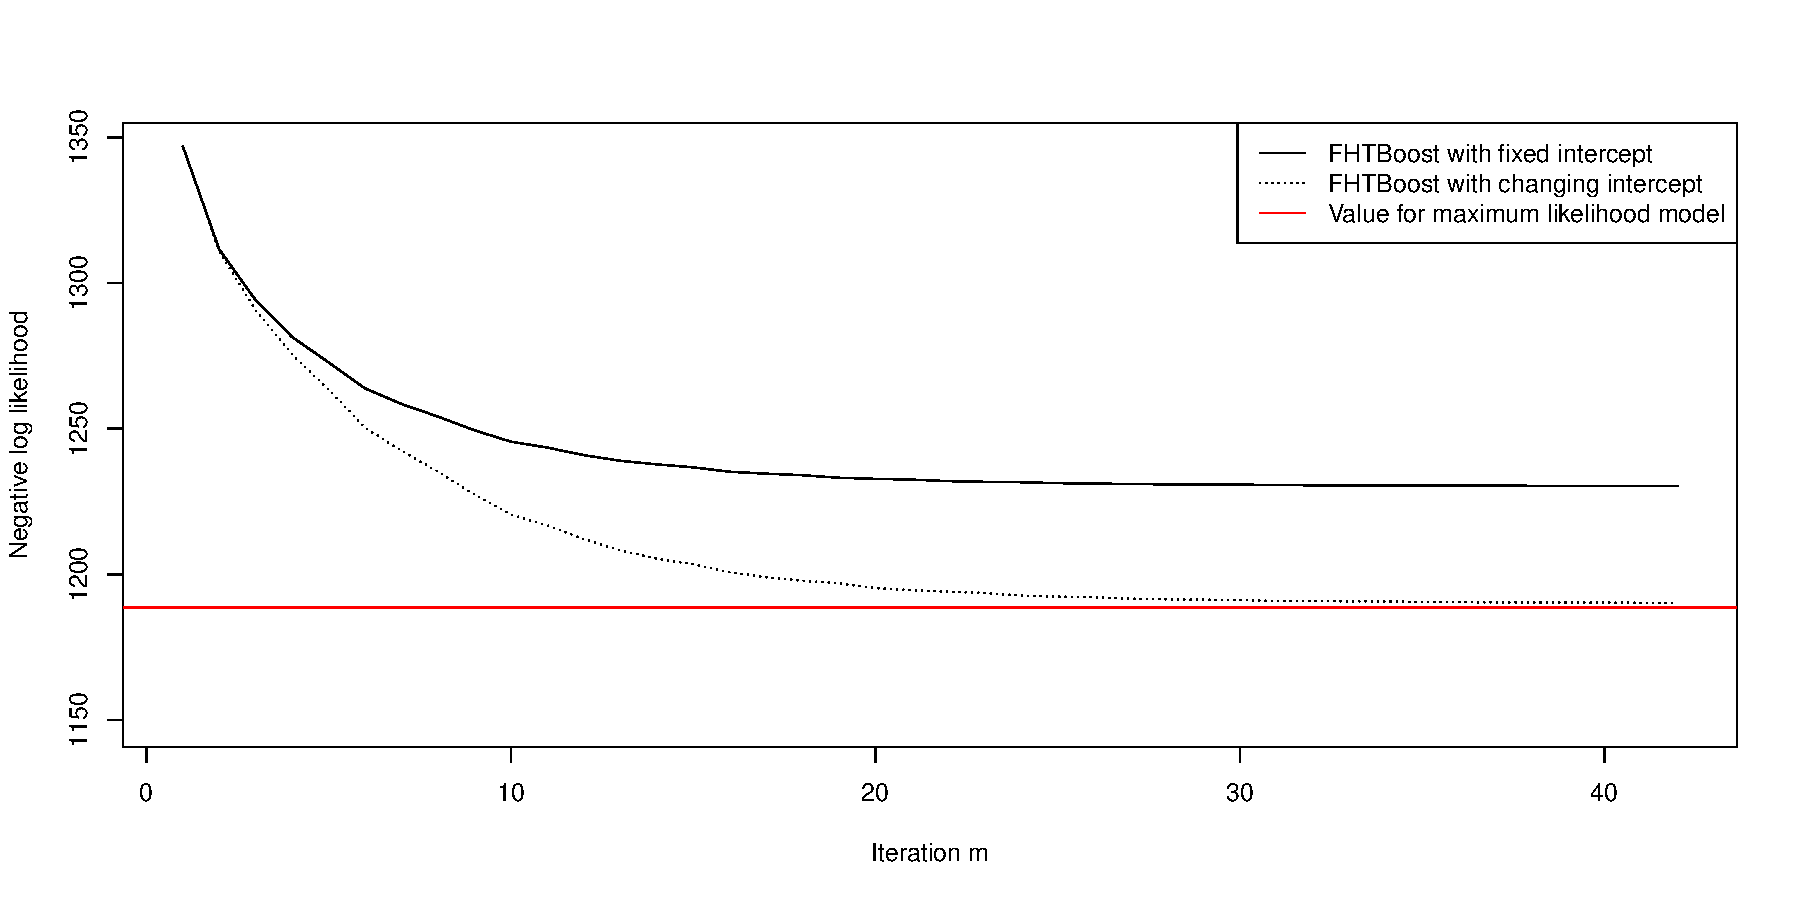
\includegraphics[scale=0.4]{figures/small_example.pdf}
\end{figure}
Figure \ref{fig:boosting-ML} shows a plot of the negative log likelihood of the data (training error) as a function of the iteration number $m$.
The solid black line shows negative log-likelihood for FHTBoost with a fixed intercept.
This is the algorithm in the previous subsection.
In this version with fixed intercept, we only estimate the intercepts $\hat{\boldeta}_0=\left(\hat{\beta}_{0},\,\hat{\gamma}_{0}\right)$ before we begin iterating, and so these intercepts are not changed in any of the boosting iterations.
The horizontal solid red line shows the negative of the maximum likelihood, obtained through numerical maximization of the joint maximum likelihood.
It is clear that FHTBoost with a fixed intercept does not reach the maximum likelihood value.
The maximum likelihood estimated intercepts are $\hat{\beta}^{\text{ML}}_{1,0}=1.98$ and $\hat{\beta}^{\text{ML}}_{2,0}=-1.02$.
FHTBoost with a fixed intercept produces estimates of the intercepts as $\hat{\beta}_{0}=1.68$ and $\hat{\gamma}^{[\mstop]}_{0}=-0.71$.
These estimated intercepts are quite off from the maximum likelihood estimates (see also Table \ref{table:ML}).

To achieve the maximum likelihood, we have to modify the algorithm to incorporate updates in the intercepts while boosting.
Some existing boosting algorithms modify the intercept, but it is not clear in the literature how these perform it.
mboost uses linear least squares base learners with an intercept.
To change the intercept in each boosting iteration, we can perform numerical maximization after updating the additive predictor, i.e. as is done initially, using the estimated additive predictors as offsets.
We are in essence treating the intercepts as nuisance parameters.
Since we will change intercepts in each iteration, we now denote intercepts with their iteration number as well.
We write $\hat{\beta}_{0}^{[m]}$ and $\hat{\gamma}_{0}^{[m]}$.
The initial intercepts are then $\hat{\beta}_{0}^{[0]}$ and $\hat{\beta}_{0}^{[0]}$.
We replace these in each iteration, with $\hat{\beta}_{0}^{[m]}$ and $\hat{\beta}_{0}^{[m]}$, which are calculated in the intercept estimated in step $m$ of the boosting algorithm.
By incorporating \textit{changing} intercepts, the algorithm was successful in recovering the maximum likelihood value and parameters.
See table \ref{table:ML} for the estimated parameter values, and graphically, in figure \ref{fig:boosting-ML}, where the convergence is plotted as a function of the number of boosting iterations.
\begin{table}\caption{Parameter values of a model which reaches ML}\label{table:ML}
\centering
\begin{tabular}{lcccccc}
\toprule
    & $\beta_{0}$ & $\beta_{1}$ & $\beta_{2}$ & $\gamma_{0}$ & $\gamma_{1}$ & $\gamma_{2}$ \\
\hline
Maximum likelihood estimate                   &    1.98 &    0.10 &    0.21 &    -1.03 &    -0.09 &     0.12 \\
FHTBoost with fixed intercept                 &    1.68 &    0.10 &    0.18 &    -0.72 &    -0.06 &     0.09 \\
FHTBoost with changing intercept              &    1.97 &    0.10 &    0.18 &    -1.02 &    -0.09 &     0.12 \\
\bottomrule
\end{tabular}
\end{table}
In step $m$, we update the additive predictor $\hat{\eta}^{[m]}_{k^{[m]}}$ by
\begin{equation*}
    \hat{\eta}^{[m]}_{k^{[m]}}\gets\hat{\eta}^{[m-1]}+\nu\cdot\hat{h}_{k^{[m]},j^{[m]}}^{[m]},
\end{equation*}
we update the intercept in the additive predictors by
\begin{equation*}
    \hat{\boldeta}_0^{[m]}\gets\hat{\boldeta}_0^{[m-1]}+\argmin_{\boldeta_0}\err\left(\boldeta^{[m]}\right).
\end{equation*}
The fact that we update the intercept in each iteration has the benefit that the resulting intercepts are the maximum likelihood intercepts \textit{with} the covariate effects estimated while boosting.
Meanwhile, for the fixed intercept, the estimated intercepts there are the maximum likelihood intercepts \textit{without} the estimated covariate effects.
\todo[inline]{This needs to be fixed}

\section{FHTBoost algorithm with changing intercept}\label{subsec:FHT-intercept}
%\begin{algorithm}
We modify algorithm \ref{algo:fhtboost} with the proposed modification with changing the intercepts in each iteration.
We replace step \ref{algostep:FHT-end} in the fixed intercept algorithm in Section \ref{algo:fhtboost} by this step, where we incorporate changing intercepts for the additive predictors in each boosting iteration.
\label{algo:fhtboost-with-intercept}
\begin{enumerate}
    \setcounter{enumi}{12}
    \item
        Find which parameter should be included in the model,
        \begin{equation*}
            k^{[m]}=\argmin_{k\in\{1,2\}}\Delta\rho_k.
        \end{equation*}
        Include this component in the final model, by updating its additive predictor,
        \begin{equation*}
            \hat{\eta}^{[m]}_{k^{[m]}}=\hat{\eta}^{[m-1]}_{k^{[m]}}+\nu\cdot\hat{h}^{[m]}_{k^{[m]},\,j^{[m]}}(x),
        \end{equation*}
        while for the other component $k\neq k^{[m]}$, set the additive predictor for this iteration to be the same as previous iteration
        \begin{equation*}
            \hat{\eta}^{[m]}_{k}=\hat{\eta}^{[m-1]}_{k}.
        \end{equation*}
        Find the best numerical constant to add to the intercept of the selected additive learner,
        \begin{equation}
            c=\argmin_c \err\left(\hat{\boldeta}^{[m]}+c\right)
        \end{equation}
        Add this $c$ to the selected parameter
        \begin{equation}
            \hat{\beta}_{k^{[m]},0}\gets\hat{\beta}_{k^{[m]},0}+c.
        \end{equation}
\end{enumerate}
%\end{algorithm}
\todo[inline]{The above needs work!}

\section{Existing work}
gamlss.cens \citep{gamlsscens}


In the next chapter, we perform a simulation study to verify that FHTBoost works to estimate FHT models.
Since we have two versions, we also compare their performance.

\section{Boosting only one parameter}
As mentioned in subsection \ref{subsec:FHT-combine}, the FHT model lends itself easily to combining genomic and clinical data, and this holds for FHTBoost as well.
There is also a straightforward way to only use one kind of covariates, i.e., only clinical covariates or only genetic covariates.
To do this, we can use the cyclical version of the algorithm, where we boost both parameters in each step, but each has its own tuning parameter.
This lets us fix the number of boosting steps of the parameter not to be boosted to 0.
In other words, we make a genomic version of FHTBoost, or $y_0$-only version of FHTBoost, by only boosting the initial level $y_0$.
This version of FHTBoost has $m_{\text{stop},1}$, corresponding to $\mu$, fixed at 0, while we perform cross-validation in the usual way to find the optimal $m_{\text{stop},2}$, corresponding to $y_0$.
Similarly, the clinical version fixes $m_{\text{stop},2}$ at 0, and tunes the other, $m_{\text{stop},1}$, corresponding to $\mu$.